\section{Aufbau}
Grundlegende Bauelemente sind zwei Platten, eine Photokathode und eine Auffängerelektrode.
Die im Verlauf des Versuches mit Photonen bestrahlte Photokathode ist zudem mit der anderen Platte über ein Strommessgerät verbunden.
Dadurch lässt sich der nun entstandene Strom messen und dieser gibt wiederum Aufschluss auf die Grenzspannung.

\begin{figure}
    \centering
    \includegraphics[width=0.5\textwidth]{bilder/müde.png}
    \caption{Schematischer Aufbau einer Messvorrichtung zur Beobachtung des Photoeffekts. \cite{skript}.} 
    \label{fig:müde1}
\end{figure}
\FloatBarrier
\subsection{Die Photozelle}
\begin{figure}
    \begin{minipage}{0.5\textwidth}
Der oben genannte Aufbau wird realisiert in einer Photozelle. In einem Vakuum befindet sich eine Photokathode die durch 
eine Metallschicht den Ansprüchen gerecht gemacht wurde. Um diese Schicht herum verläuft ein dünner Draht der so die Funktion der Anode 
erfüllt. Der Draht und die Photokathode liegen parallel zueinder, das heißt an jeder Stelle teilen sich Kathode und Anode einen gemeinsamen Normalenvektor.
Die Messreihen verlangt, dass eine externes Feld in diesem Raum angelegt wird um den Transport der Photoelektronen und somit 
messbare Ergbenise, zu erleichtern.  Dafür ist der Draht und die Photokathode mit einem einstellbaren Generator verbunden was es also möglich macht, 
das gewünschte Feld im Glaskörper zu erzeugen. Zusätzlich misst ein weiteres Messgerät den fließenden Strom welcher auf Grund 
der Kontaktlosigkeit nur durch eben ausgelösten Elektronen entstehen kann. 
     \end{minipage}
\hfill
    \begin{minipage}{0.5\textwidth}
        \centering
        \includegraphics[width=0.9\textwidth]{bilder/sehrmüde.png}
        \captionsetup{justification=centering}
    \captionof{figure}{Schematischer Aufbau \\ einer Messvorrichtung zur Beobachtung \\ des Photoeffekts. \cite{skript}.} 
    \label{fig:sehrmüde}
    \end{minipage}
\end{figure}

\subsection{Monochromatisches Licht}
Es bietet sich für die Auswertung an, die Photozelle nur mit Licht einer bekannten Wellenlänge zu bestrahlen.
Dazu müssen die einzelnen Spekrallinien, erzeugt von einer Spektrallampe, räumlich von einander getrennt werden. 
Die Umsetzung dieser Trennung erfolgt durch Linsen und einem Spalt, der das Licht möglichst scharf auf ein Gradsichtprisma lenkt.
Das Prisma bricht anschließend das Licht unterschiedlicher Wellenlängen, gemäß dem Snellius'schen Brechungsgesetz unterschiedlich 
stark wodurch nacher die gewünschte Farbe mit räumlichen Abstand von der Photozelle eingefangen werden kann.
\begin{figure}
    \centering
    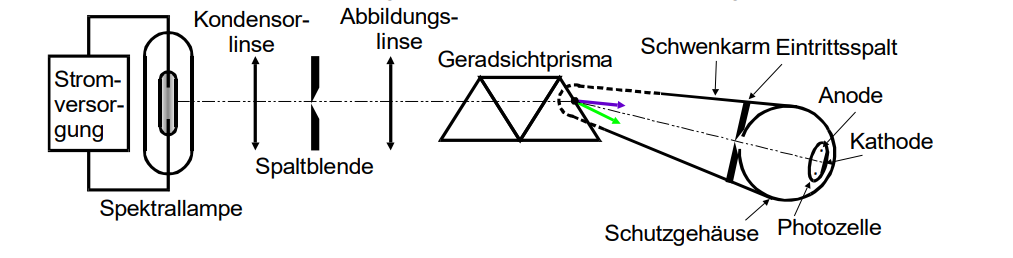
\includegraphics[width=0.5\textwidth]{bilder/licht.png}
    \caption{Schematische Darstellung der Brechung und Fokusierung des Lichts aus einer Spektrallampe mit anschließendem Einfall in eine Photozelle \cite{skript}.} 
    \label{fig:müde}
\end{figure}

\begin{figure}
    \centering
    \includegraphics[width=0.5\textwidth]{bilder/bisschenmüde.png}
    \caption{Finaler Aufbau als Schaltplan der verschiedenen Elemente zur empirischen Ermittlung der Phänomene des Photoeffekts \cite{skript}.} 
    \label{fig:müde}
\end{figure}
\section{Durchführung}
Die verschiedenen Messreihen werden für vier Wellenlängen durchgeführt. Diese sind in der Tabelle \ref{tab:tab5} angegeben. %maybe reinschreiben???
Dies verlangt, dass die Messung mit der Einstellung des Primas und Positionierung der Photozelle beginnt. 
Nun werden am Generator Spannungen im Intervall $\{\SI{-2}{\volt},... ,\SI{2}{\volt}\}$ erzeugt und gemessen mit Messabständen, die sich im Bereich um die $\SI{0}{\volt}$ herum erhöhen.
Der beobachtete Photonenstrom $I_{ph}$ wird dabei gemessen und notiert. Um eine höhere Messgenauigkeit zu erreichen empfiehlt es sich externe Lichtquellen, die
auch in die Photozelle einfallen könnten zu verdunkel oder auszuschalten. Außerdem bietet es sich an grobe Berührungen am Tisch gänzlich zu vermeiden, 
denn das Ampermeter reagiert sehr empfindlich auf alle aüßeren Einflüsse, auch Erschütterungen.
\\
\newline
Die letzte Messreihe behandelt ausschließlich das gelbe Licht, also eine Wellenlänge von $577\si{\nano\meter}$ und $579 \si{\nano\meter}$ wobei jedoch ein 
Spannungsintervall von $\{\SI{-20}{\volt},... ,\SI{20}{\volt}\}$ angelegt wird. Die jetzt große, negative Spannung macht es möglich, nach Umschalten auf negative Werte am Ampermeter,
einen negativen Stromfluss $I_{ph}$ zu messen. Dieser wird entsprechend notiert. 
